%!TEX program = xelatex
%%%%%%%%%%%%%%%%%%%%%%%这是导言部分的开始%%%%%%%%

%========= 导言部分声明文档的类型=================
\documentclass{article}

	%=========导言部分可可以加载宏包=================
	\usepackage{amsmath}                % 数学公式排版宏包
	\usepackage{amssymb}                % 数学符号命令宏包
	\usepackage{amsthm}                 % 数学定理宏包
	\usepackage[UTF8]{ctex}             % 中文输入宏包
	\usepackage[a4paper]{geometry}      % 页面设置宏包
	\usepackage{setspace}               % 行间距宏包
	\usepackage{graphicx}               % 图片宏包
	\usepackage{listings}               % 代码宏包
	\usepackage{color}					% 颜色宏包
	\usepackage{xcolor}                 % 颜色处理宏包
	\usepackage{float}                  % 浮动对象式样宏包
	\usepackage{fontspec}
	\usepackage{enumerate}				% 列举编号包
	
	%=========页面设置==============================
	\geometry{left=1cm,right=1cm,top=1cm,bottom=2cm}
	\onehalfspacing
	\setlength\parindent{0em}

	%=========代码格式设置============================
	\definecolor{dkgreen}{rgb}{0,0.6,0}
	\definecolor{gray}{rgb}{0.5,0.5,0.5}
	\definecolor{mauve}{rgb}{0.58,0,0.82}
	% \setmonofont{Consolas}
	\lstset{
		numbers = left, 	
		numberstyle = \color{gray}, 
		keywordstyle = \color{blue},
		commentstyle = \color{dkgreen}, 
		stringstyle = \color{mauve},
		basicstyle = \ttfamily,
		breaklines = true,
		frame = shadowbox, % 阴影效果
		rulesepcolor = \color{ red!20!green!20!blue!20} ,
		escapeinside = ``, % 英文分号中可写入中文
		xleftmargin = 2em,xrightmargin=2em, aboveskip=1em,
		framexleftmargin = 2em
	} 

%=========导言部分可以定义标题信息===============
\title{组会报告}
\author{徐益}
\date{\today}
%%%%%%%%%%%%%%%%%%%%%%%这是导言部分的结束%%%%%%%%%

%%%%%%%%%%%%%%%%%%%%%%%这是正文部分的开始%%%%%%%%%
\begin{document}

%=========生成标题================================
\maketitle

%=========开始正文的输入==========================

%===========第一节=================
\section{工作内容}
1. 修改仿真报告;

2. 编写数据采集程序并测试;

3. 学习LDPC低时延译码方案。

%===========第一节=================
\section{改写仿真报告}

%===========第二节=================
\section{数据采集程序测试结果}
\subsection{不进行写入操作}
\begin{figure}[H]
	\centering
	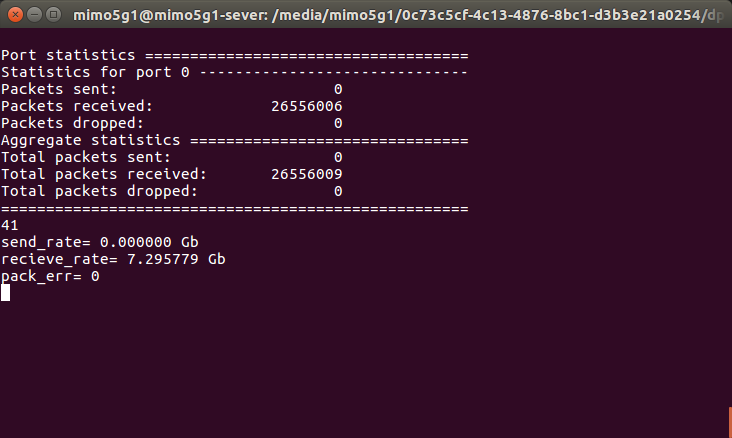
\includegraphics[width = .8\textwidth]{rate1.png}
	\caption{不进行写入操作时的速率}
\end{figure}
\begin{figure}[H]
	\centering
	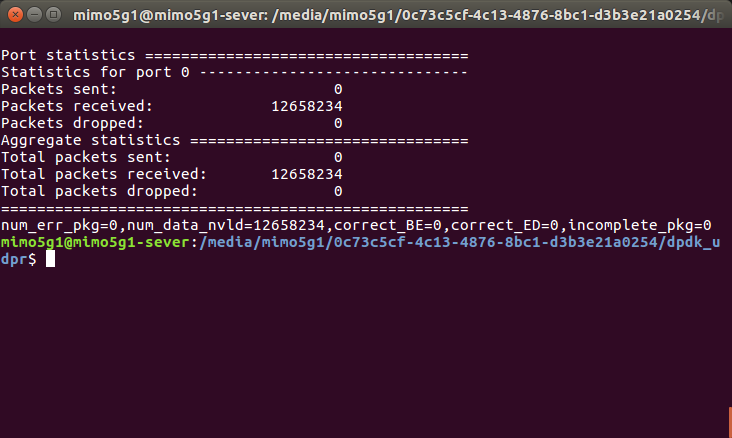
\includegraphics[width = .8\textwidth]{res1.png}
	\caption{不进行写入操作时的结果}
\end{figure}
\subsection{通过fprintf写入}
\begin{figure}[H]
	\centering
	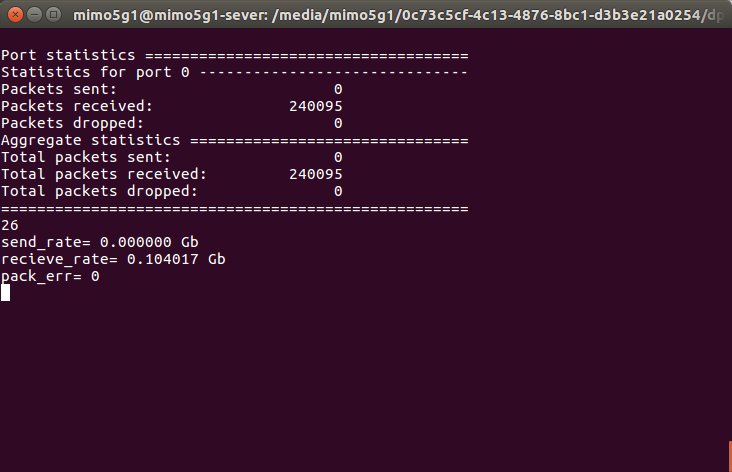
\includegraphics[width = .8\textwidth]{fprintfrate.png}
	\caption{通过fprintf写入时的速率}
\end{figure}
\subsection{通过fwrite写入}
\begin{figure}[H]
	\centering
	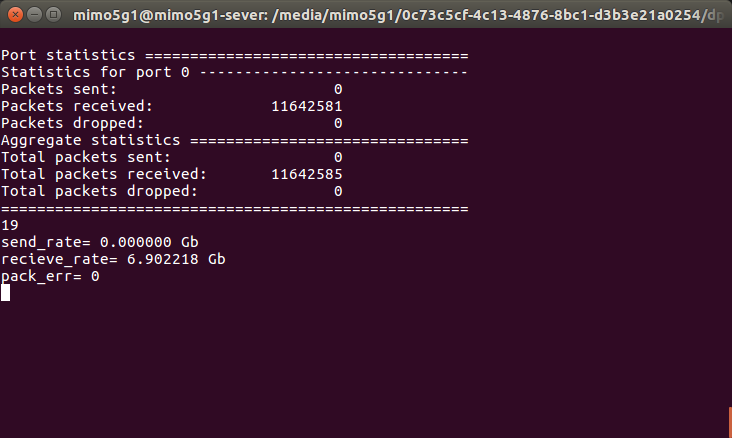
\includegraphics[width = .8\textwidth]{fwriterate.png}
	\caption{通过fwrite写入时的速率}
\end{figure}
\begin{figure}[H]
	\centering
	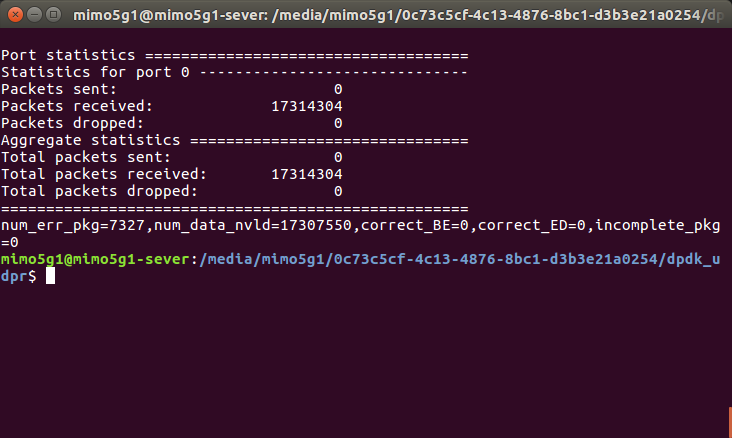
\includegraphics[width = .8\textwidth]{fwriteres.png}
	\caption{通过fwrite写入时的结果}
\end{figure}
\subsection{降低速率后通过fwrite写入}
\begin{figure}[H]
	\centering
	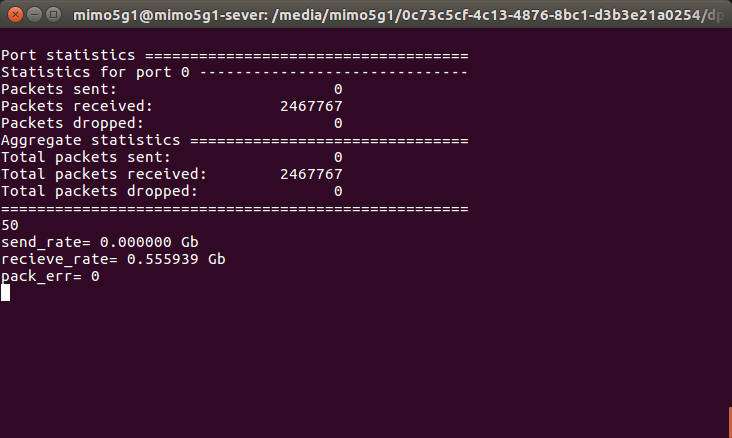
\includegraphics[width = .8\textwidth]{lowrate.png}
	\caption{降低速率后通过fwrite写入时的速率}
\end{figure}
\begin{figure}[H]
	\centering
	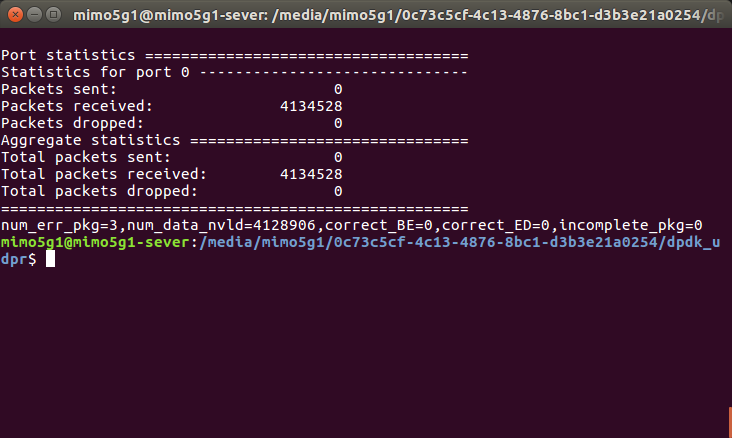
\includegraphics[width = .8\textwidth]{lowres.png}
	\caption{降低速率后通过fwrite写入时的结果}
\end{figure}

%===========第三节=================
\section{学习LDPC低时延译码方案}



%===========第四节=================
% \section{仍存在的问题}


%===========下周计划=================
% \section{下阶段计划}
% 1. 继续完成仿真报告

\end{document}
%%%%%%%%%%%%%%%%%%%%%%%这是正文部分的结束%%%%%%%%%%%%